%-----------------------------------------------------------------------------
%
%               Template for sigplanconf LaTeX Class
%
% Name:         sigplanconf-template.tex
%
% Purpose:      A template for sigplanconf.cls, which is a LaTeX 2e class
%               file for SIGPLAN conference proceedings.
%
% Guide:        Refer to "Author's Guide to the ACM SIGPLAN Class,"
%               sigplanconf-guide.pdf
%
% Author:       Paul C. Anagnostopoulos
%               Windfall Software
%               978 371-2316
%               paul@windfall.com
%
% Created:      15 February 2005
%
%-----------------------------------------------------------------------------


\documentclass[preprint]{sigplanconf}

% The following \documentclass options may be useful:

% preprint      Remove this option only once the paper is in final form.
% 10pt          To set in 10-point type instead of 9-point.
% 11pt          To set in 11-point type instead of 9-point.
% numbers       To obtain numeric citation style instead of author/year.

\usepackage{amsmath}
\usepackage{subfig}
\usepackage{balance}
\usepackage[normalem]{ulem}
\usepackage{graphicx}
\usepackage{caption}
%\usepackage{subfig}
\usepackage{array}
\usepackage{amsmath}
\usepackage[algosection,ruled,linesnumbered,vlined]{algorithm2e}

%\usepackage{fancyhdr}
%\usepackage[normalem]{ulem}
%\usepackage[hyphens]{url}

%\usepackage{hyperref}
%\hyphenation{op-tical net-works semi-conduc-tor}
%\usepackage{epsfig,endnotes}
%\usepackage{subcaption}
%\usepackage{url}

%\usepackage{color}
\usepackage{multirow}
%\usepackage{amsmath,bm}
%\usepackage[section]{algorithm}
%\usepackage{algorithmic}
\usepackage{makecell}
%\usepackage{setspace}
%\usepackage[square,sort,comma,numbers]{natbib}
%\renewcommand{\algorithmicrequire}{\textbf{Input:}}
%\renewcommand{\algorithmicensure}{\textbf{Output:}}
%\renewcommand{\thefootnote}{\arabic{footnote}}
\usepackage[marginal]{footmisc}
\newcommand{\ignore}[1]{}
\newcommand{\tabincell}[2]{\begin{tabular}{@{}#1@{}}#2\end{tabular}}

\newcommand{\cL}{{\cal L}}

\begin{document}

\special{papersize=8.5in,11in}
\setlength{\pdfpageheight}{\paperheight}
\setlength{\pdfpagewidth}{\paperwidth}

\conferenceinfo{CONF 'yy}{Month d--d, 20yy, City, ST, Country}
\copyrightyear{20yy}
\copyrightdata{978-1-nnnn-nnnn-n/yy/mm}
\copyrightdoi{nnnnnnn.nnnnnnn}

% Uncomment the publication rights you want to use.
%\publicationrights{transferred}
%\publicationrights{licensed}     % this is the default
%\publicationrights{author-pays}

\titlebanner{banner above paper title}        % These are ignored unless
\preprintfooter{short description of paper}   % 'preprint' option specified.

\title{Title Text}
\subtitle{Subtitle Text, if any}

\authorinfo{Name1}
           {Affiliation1}
           {Email1}
\authorinfo{Name2\and Name3}
           {Affiliation2/3}
           {Email2/3}

\maketitle

\begin{abstract}
\input{0-abstract}
\end{abstract}

\category{CR-number}{subcategory}{third-level}

% general terms are not compulsory anymore,
% you may leave them out
\terms
term1, term2

\keywords
keyword1, keyword2

%\section{Introduction}
\section{Introduction}
\label{sec:intro}

% 1.deep learning and convolutional neural network are more and more applied in daily-life, and in smart-phone,embedded system has some applications.
% 2.there some question in embedded system trained and more and more application or previous works for android and ios.
% 3. there are some state-of-the-art cnn, accuracy is not good , the higher number of trained set is more high accuary, and

%4.in traditional machine learning, the incremental learning,cloud as assistance
In the recent decade, deep neural networks have a prominent performance in many high-impact machine learning applications. These include speech recognition~\cite{hinton2012deep},object classification~\cite{K-2012-imagenet,sermanet2013overfeat},image caption generation~\cite{vinyals2015show,karpathy2015deep} and semantic segmentation~\cite{semantic-1,semantic-2,semantic-3}. As the size of data sets is increasingly large, so do the number of parameters in deep neural networks for the sake of comprehending the enormous amount of useful information contained in data sets, such as some modern networks like AlexNet~\cite{K-2012-imagenet}(60M parameters), and VGG-16~\cite{vgg-16}(130M parameters).

Large DNN models are very powerful but energy-consumed and time-consuming, especially during training~\cite{K-2012-imagenet,vgg-16}. Thus training these network on wearable, smartphones and Internet-of-Things devices are impractical. As a result, prominent examples of deep learning applied on smart-phones(e.g.,speech recognition) are primarily cloud-supported. Hence increasingly, these networks are trained on industrial-sized clusters~\cite{le2013building} or high-performance graphics processing units(GPUs)~\cite{catanzaro2013deep,hauswald2015djinn}. What's more, in the actual industry, there is a significant class of emerging internet services known as intelligent personal assistants(IPAs), like Apple Siri, Google Now, Microsoft Cortana and Amazon Echo. However, the cloud-assisted pattern introduces important negative side-effects: 1) it raises an issue with regard to user privacy~\cite{harris2015your} as some sensitive data (e.g.,audio or video) is processed in the cloud by a third party; and 2)it only works when sufficient bandwidth is feasible and suffers artificial delays through network traffic~\cite{kosnerclient}(i.e., latency,throughput).

To solve the above problems, several kinds of emerging solutions have been proposed. A kind of solutions is to directly train small models for the on-device classification; however, these tend to observably impact accuracy~\cite{chun2009augmented}, leading to customer discontent. Another kind of solutions is to compress pre-trained deep networks, which have been trained on industrial-sized clusters(server-side). More and more researchers are studying in this direction. Recent work by Denil et.al.~\cite{denil2013predicting} proves that there exists a amazingly large amount of redundancy among the weights of deep neural networks. The authors point out that a slight amounts of the weights are adequate to reconstruct the entire network. Accordingly, through pruning the redundant, non-informative weights, the size of large trained neural networks can be reduced up to 50X~\cite{han2015learning,han2015deep} without any loss of accuracy. More recently, other various methods based on low-rank decomposition~\cite{denton2014exploiting}, vector quantization~\cite{gong2014compressing}, hashing techniques~\cite{chen2015compressing}, circulant projection~\cite{cheng2015fast}, tensor train decomposition~\cite{novikov2015tensorizing}, and network binarization~\cite{courbariaux2014training,courbariaux2015binaryconnect} were proposed without significant drop in the prediction accuracy.

In a word, Compression is an effective way to transfer clumsy neural networks from server-side into mobile-side. A obvious advantage here is that these compression schemes may actualize local processing and storage of neural networks, and to some extent, protect user privacy as well as avoid the response delays and energy consumption from bandwidth restrictions. However, in these pattern, the neural networks deployed on mobile devices is fixed and can not relearn against reality.

As increasing works have successfully achieve the application of deep neural networks without compression on mobile devices~\cite{latifi2016cnndroid,oskouei2015gpu,brandle2015face,yanai2016efficient,mittal2016spotgarbage,cnnforandroid}. It is imperative to further enhance the interaction with the mobile end user. For example,

In this paper, we propose a concept of application frameworks 

Overall, this paper makes the following contributions.




%ʵ�������Լ�һЩ����

% the overarching goal of this paper is
%spurious uploads.
%facilitating its usage in resource constrained smartphone.
%Thus, the solution should try to avoid uploading every image, and rather process them on the phone itself.
%and it should send minimal information such as GPS-coordinates/ severity of garbage and optionally, a segmented region of the image containing the garbage over the network.
%according the prediction result,  give a severity of error recognition. we will do some work in accordance with it.

%This compression scheme may achieve local processing of mobile phones, to a certain extent, to protect the user's privacy and security to avoid bandwidth constraints, but this solidified the model results, no learning ability
%���ܴ���Խ��Խ���Ŭ����cnn�����ƶ��豸�У����ǽ�����ʹ���Ѿ�ѵ���õ�ģ�ͣ�������ʵ���ƶ��˵���ѵ��ѧϰ��
%Although there are more and more efforts to deploy CNN to mobile devices, but only using trained models, but can not achieve mobile terminal retraining study.
%In addition, 




As the most representative networks like AlexNet(240MB), and VGG-16(520MB), are too large to deploy on mobile devices and embedded systems.


Deploying convolutional neural networks(CNNs) for various intelligent tasks on embedded and mobile devices(e.g., smartphones) is obtaining more and more attention.
 
\section{Background And Motivation}
\label{bkg_motivation}

\subsection{Background}
\label{bkg}



\subsection{Personalized Features \textit{\textbf{\large}}}
\label{feature}
In this paper, we consider five kinds of contextual information as follows:




\begin{itemize}
    \item \textbf{$L$:} 

    \item \textbf{$D, H$:} 

    \item \textbf{$Wf$:} 

    \item \textbf{$B, C$:} 

    \item \textbf{$LP$:} 
\end{itemize}


 Table~\ref{tbl: acronym} summarizes the features considered. What's more, the table also give the description of acronyms to be used in the following passage.


\subsection{Traditional Bayesian Algorithm \textit{\textbf{\large}}}
\label{traditional_algorithm}
 The traditional Bayesian algorithm is shown in Equation~\ref{eq: prediction}, we calculate each App's prediction score given the context by multiplying the CPDs(the conditional probability distribution) of the App and each context. Then the top scored Apps are the final predictions. The CPD $P(A | C)$ denote that the probablity of launching an App under the condition of the last used App. The meaning of the other three CPDs is similar.


\begin{table}[t]
\setlength{\tabcolsep}{1.2em}
\scriptsize
  \centering
  \caption{Notation used in this paper.}
  %\begin{tabular}{|p{3cm}<\centering||p{1.2cm}<\centering|p{2cm}<\centering|p{2cm}<\centering|p{2cm}<\centering|}
  \begin{tabular}{c|c}
     \hline
     Symbol & Description \\
     \hline
     \hline
     $L$ & the location  \\
     $D$ & day of week  \\
     $H$ & hour of day  \\
     $Wf$ & the rate level of wifi  \\
     $B$ & the battery level  \\
     $C$ & a flag whether the battery is being charged  \\
     $LP$ & the latest used App  \\
     $A$ & the App   \\
     $CPD$ & the conditional probability distribution  \\
     \hline
   \end{tabular}
 \label{tbl: acronym}
 \vspace{-0.1in}
\end{table}


\begin{equation}
\footnotesize
\label{eq: prediction}
    Socre(A) = P(A | C) \times P(A|D,H,L) \times P(A|W) \times P(A|U)
\end{equation}


 It is intuitive that we should consider as many records (i.e., training data) as possible in order to achieve high prediction accuracy. Because the penalty for using small training sets is over fitting: while in-sample performance may be excellent, The previous work on App prediction has tended to make use of a lot of training samples. However, we need to take the specific area of application into account. Using machine learning algorithm to predict next App that smartphone user will be used, we have to consider that user behavior patterns can have a change gradually. Thus, using long-term training sets can reduce prediction accuracy instead.


\begin{figure}[t]
    \centering
    \begin{tabular}[t]{c}
        \subfloat[]{
\includegraphics[width=0.55\columnwidth]{fig/U1_5_5_frequency.eps}}
        \subfloat[]{
\includegraphics[width=0.55\columnwidth]{fig/U2_5_5_frequency.eps}}
    \end{tabular}
    \centering
    \begin{tabular}[t]{c}
        \subfloat[]{
\includegraphics[width=0.55\columnwidth]{fig/U3_5_5_frequency.eps}}
        \subfloat[]{
\includegraphics[width=0.55\columnwidth]{fig/U4_5_5_frequency.eps}}
    \end{tabular}
    \caption{(a)(b)(c)(d)indicate that the used ratio of most frequently used 8 Apps on four different smartphone users.}
    \label{fig: motivation}
    \vspace{-0.1in}
\end{figure}


To demonstrate our inference, we have an analysis of most frequently used Apps. As shown in Figure~\ref{fig: motivation}, we count the used ratio of 8 Apps every 5 weeks. The number of tag such as 2 indicates the second five- weeks in the upper right corner. The 8 Apps are the most frequently used Apps for the user. The used ratio of every App varies with time. Thus, in term of the used frequency of Apps, we conclude the conclusion that user behavior pattern of using Apps varies with time.

\begin{figure}[t]
    \centering
    \begin{tabular}[t]{c}
        \subfloat[]{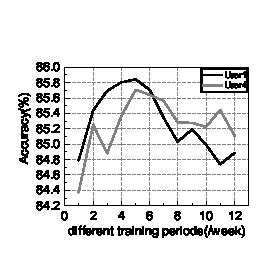
\includegraphics[width=0.55\columnwidth]{fig/U1_U4.eps}}
        \subfloat[]{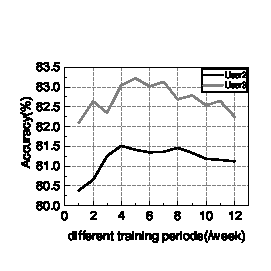
\includegraphics[width=0.55\columnwidth]{fig/U2_U3.eps}}
    \end{tabular}
    \caption{(a)(b)indicate that the changing trend of prediction accuracy along with increasement of the size of training sets.}
    \label{fig: 2_week_test_accuracy}
    \vspace{-0.1in}
\end{figure}



Also, we demonstrate the inference from the view of the prediction accuracy. We explore the impact of the amount of training data ranged from one week to twelve weeks on the prediction accuracy. There are two schemes to get prediction accuracy from data set. The two schemes are shown in Figure ~\ref{fig: train_test_flow}. In Scheme 1, training periods and test periods alternately present and they have no overlap on the time dimension. From Figure ~\ref{fig: train_test_flow}(b), we can find that there exists overlapping parts on the time dimension in Scheme 2. And in Scheme 2, there is no time interval in two adjacent test periods. In both two schemes, after the $i_{th}$ training period, we get prediction accuracy from the corresponding $i_{th}$ test period based on the model trained in the $i_{th}$ training period. In the Equation~\ref{eq: user_acc}, $ave_acc_user$(the average value of all the average accuracy in every test period) represent the prediction accuracy on a user and $acc\_each$ is the prediction accuracy each test. $n_{1}$ is the number of test periods in dataset and $n_{2}$ is the times of test in each test period.


\begin{equation}
\footnotesize
\label{eq: user_acc}
ave\_acc\_user=\sum_{i=1}^{n_{1}} \sum_{j=1}^{n_{2}} acc\_each
\end{equation}


In this paper, we adopt


\begin{figure}[t]
    \centering
    \begin{tabular}[t]{c}
        \subfloat[]{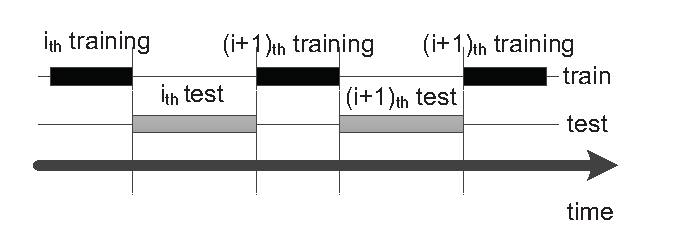
\includegraphics[width=0.95\columnwidth]{fig/train_test_flow_scheme1.eps}}
    \end{tabular}
    \centering
    \begin{tabular}[t]{c}
        \subfloat[]{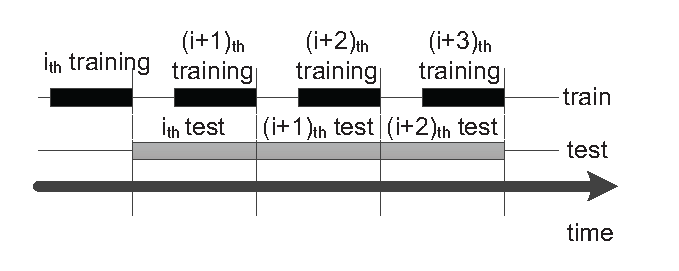
\includegraphics[width=0.95\columnwidth]{fig/train_test_flow_scheme2.eps}}
    \end{tabular}
        \caption{(a) (b) represents two different schemes to get prediction accuracy from data set. (a) describes Scheme 1 and (b) describe Scheme 2.}
    \label{fig: train_test_flow}
\end{figure}


As shown in Figure~\ref{fig: 2_week_test_accuracy}, the experimental results are based real traces collected from the 9 participants. And the k is set at 5. From the Figure~\ref{fig: 2_week_test_accuracy}, we can see that the prediction accuracy will rise at the beginning, but it will drop then. Namely, the accuracy is saturated at certain point from one week to twelve week. Therefore, the long-term training data does not necessarily achieve higher accuracy. Heuristically, it is because mobile users may install new Apps and have changed their behavior patterns(e.g. preferences) slightly. On the other hand, more records(i.e., training data) more time required to make prediction.


We also conclude from Figure~\ref{fig: 2_week_test_accuracy} that the positions the saturation points varies greatly on different mobile users. So it is necessary to have s adaptive scheme to adjust the amount of training data. However, it is difficult to select the optimal amount of training data directly. The work flow of App prediction is training-prediction-retraining-reprediction. We fixed the amount of training data and adjust the time span of the period of prediction instead. Because the precision accuracy is easily obtained in the period of prediction. We can adjust the time span based on the prediction accuracy.


From Figure~\ref{fig: motivation,fig: 2_week_test_accuracy}, we get two observations that provide useful insights into the design of our algorithm.


\textbf{Observation 1:}User behavior pattern of using Apps varies with time. And the recent used Apps are more useful to predict the next used Apps.


\textbf{Observation 2:}For different smartphone users, the optimal amounts of training data id different. Therefore, we propose an adaptive algorithm to solve the problem.

%Instead, select an approximate time span of p


%On the one hand, more records(e.g. train

%Different size of training sets are chosento measure the influence of the size of training sets on prediction accuracy. We do our experiments on nine smartphone users. According to the time span of training sets, the training sets is classified into twelve categories. The time span of twelve categories is from one week to twelve week. The experimental results are shown in the Figure~\ref{fig: 2_week_test_accuracy}.

%we first count the 8 Apps of most frequently used Apps from the whole datasets from different users. Then, the used ratio


%In addition, predicting mobile application usage with contextual information has been studied for a long time. Ke Huang et al~\cite{PredictByContextInfo} study bayes based method and linear model to conduct prediction. And ~\cite{PredictTLB} proposes a prediction-guided multi-grain TLB design that uses a superpage prediction mechanism to avoid multiple lookups in the common case.

%As a result, processes are terminated directly if there is no enough memory space, which may degrade user satisfaction.


\subsection{Adjusting the time span of the prediction period adaptively \textit{\textbf{\large}}}
\label{measure_study}
%\subsection{Launching Apps with Swapping: \textit{\textbf{\large Not}} Just Read I/O!}
%\label{measure_study}
From the above, choosing an approximate amount of training data can not only improve the prediction accuracy but also reduce the time required to train the prediction model. Because the prediction accuracy can be obtained in the period of prediction, we choose an a dynamic time span of prediction period instead of a dynamic amount of training data. We thus propose a strategies based on the minimization of the prediction error. It can be considered as \emph{early stopping}.


\emph{Early stopping}: In machine learning, early stopping is a form of regularization used to avoid over-fitting when training a learner with an iterative method, such as gradient descent. Such methods update the learner so as to make it better fit the training data with each iteration. Early stopping rules provide guidance as to how many iterations can be run before the learner begins to over-fit.


We have used the strategy of \emph{early stopping} to achieve the adaptive time span of prediction periods. The detailed description is as follows. After training with a fixed amount of training data, the achieved model by training is used to predict the Apps that will be used next. At this time, an approximate time span of prediction periods need to be considered. Too long time span of prediction periods can make the prediction accuracy decreased. But too short time span of prediction periods can increase the training costs(i.e., more training times are needed). In our strategy of \emph{early stopping}, we first need to selected an initial time interval(e.g., two weeks). In the strategy, the shortest time span of prediction period is one week(i.e., the first week in the two weeks). The rest of the prediction time can be dynamically adjusted. Except from the first week, the average precision accuracy(acc\_day) of the whole prediction period need to be calculated with every passing day. At the same time, the average prediction accuracy(acc\_week) of the whole prediction period also need to be calculated with every passing week. But considering to improve the final prediction accuracy, the maximal acc\_week(max\_acc\_week) is chosen as a baseline.


Intuitively, the acc\_week is more stable than the acc\_day, and the it is more representative than the acc\_day. Thus, with every passing day, we calculate acc\_day, max\_acc\_week and compare acc\_day and max\_acc\_week. Provided the ratio of acc\_day and acc\_week is less than the threshold that we set, we have a time penalty for time span of prediction period(i.e., reducing the time span of prediction period). In the beginning, we have selected an initial time interval of two week. Excluding the first week, the second week is chosen as a baseline. When the prediction accuracy is too low, the time span of prediction period can be reduced on the basis of the baseline.


\begin{algorithm}[!t]
\SetKwInOut{Input}{Input}\SetKwInOut{Output}{Output}
\footnotesize
 \Input{$L$: an empty list;
        $TS$: a fixed time span;
        $Thres1$: a number between 0 and 1;
        $Thres2$: a number between 0 and 1;}
 \Output{$ave\_acc_{total}$: the average prediction accuracy in the whole prediction period;}
 \medskip
 $n\_predict$ $\leftarrow$ 0\;
 $sum\_accuracy$ $\leftarrow$ 0\;
  \For{each $TS$ in the firstweek of the prediction period}{
    Predict next used Apps and get the prediction accuracy $P$\;
    $n\_predict$ $\leftarrow$ $n\_predict$+1\;
    $sum\_accuracy$ $\leftarrow$ $sum\_accuracy$+$P$\;
    \If{$Sum$ is an integer multiple of one day}{
        Add the tuple ($n\_predict$,$sum\_precision$) into list $L$\;
        $n\_predict$ $\leftarrow$ 0\;
        $sum\_accuracy$ $\leftarrow$ 0\;
    }
  }
  $RS$: the rest of prediction period;
  $RS$ $\leftarrow$ the time of one week;
  $n\_predict$ $\leftarrow$ 0\;
  $sum\_accuracy$ $\leftarrow$ 0\;
  $flag$: a flag on whether to increase the time of prediction period\;
  $flag$ $\leftarrow$ \emph{True}
  \While{$flag$}{
      \For{each $TS$ in $RS$}{
        Predict next used Apps and get the prediction accuracy $P$\;
        $n\_predict$ $\leftarrow$ $n\_predict$+1\;
        $sum\_accuracy$ $\leftarrow$ $sum\_accuracy$+$P$\;
        \If{$Sum$ is an integer multiple of one day}{
            Add the tuple ($n\_predict$,$sum\_precision$) into list $L$\;
            $n\_predict$ $\leftarrow$ 0\;
            $sum\_accuracy$ $\leftarrow$ 0\;
            Calculate average accuracy $ave_acc$ according to $L$\;
            Get the maximal accuracy $max_acc$ in the first one,two,... of prediction period
            \If{$ave\_acc$ < $max_acc$ $\times$ $Thres1$}{
                Have a penalty for $ave\_acc$(lowering the value)\;
            }
        }
      }
      Calculate average accuracy $ave_acc$ according to $L$\;
      Get the maximal accuracy $max_acc$ in the first one,two of prediction period\;
      \If{$ave\_acc$ > $max\_acc$ $\times$ $Thres2$}{
        Have an award for $RS$ (add the value)\;
      }
      $flag$ $\leftarrow$ \emph{False}\;
  }
  Calculate $ave\_acc_{total}$ according to $L$\;
  \Return $ave\_acc_{total}$;
  \caption{\textsc{Early Stopping Algorithm}}
 \label{alg: early stopping}
 \vspace{-0.2in}
\end{algorithm}


In the Algorithm\ref{alg: early stopping}, the penalty function \emph{penal\_func} is the key. We have tried to use different formula. After a lot of experiments, we choose Formula\ref{eq: penalty_function} as our final penalty function. In Formula\ref{eq: penalty_function}, $threshold$ is a number between 0 and 1 and $a$ is a parameter. Heuristically, the rate of growth of the logarithmic function value is more and more gentle, which will effectively avoid certain accidental factors to reduce the time interval between two adjacent training.

\begin{equation}
\footnotesize
\label{eq: ratio_function}
ratio=\frac{\sum_{i=1}^n each\_acc}{n \times max\_ave\_acc}
\end{equation}


\begin{equation}
\footnotesize
\label{eq: penalty_function}
    penalty=1+\frac{log(threshold)-log(ratio)}{log(a)}
\end{equation}


\begin{figure}[t]
    \centering
    \begin{tabular}[t]{c}
        \subfloat[]{
\includegraphics[width=0.55\columnwidth]{fig/A00_trainingtimes.eps}}
    \end{tabular}
    \caption{(a)(b)indicate that the changing trend of prediction accuracy along with increasement of the size of training sets.}
    \label{fig: training_times}
    \vspace{-0.1in}
\end{figure}


As shown in Figure\ref{fig: training_times}, our adaptive method nearly reduce half of the training times with flexible prediction period than using fixed prediction period(two weeks). In addition, in terms of the accuracy, the adaptive method nearly obtains the same prediction accuracy and even has an improvement for some users. The accuracy result of comparison is listed in Table \ref{tbl: adaptive_accuracy}.



\begin{table}[t]
\setlength{\tabcolsep}{.3em}
\scriptsize
  \centering
  \caption{the result of accuracy comparison between our adaptive method and adopting fixing prediction period method.}
  %\begin{tabular}{|p{3cm}<\centering||p{1.2cm}<\centering|p{2cm}<\centering|p{2cm}<\centering|p{2cm}<\centering|}
  \begin{tabular}{|c|c|c|c|c|c|c|c|c|c|}
     \hline
      \multirow{2}{*}{User} & \multirow{2}{*}{Strategy} & \multicolumn{7}{c|}{training weeks(/week)} & \multirow{2}{*}{avg} \\
      \cline{3-9}
      & & \tabincell{c}{2} & \tabincell{c}{3} & \tabincell{c}{4} & \tabincell{c}{5} & \tabincell{c}{6} & \tabincell{c}{7} & \tabincell{c}{8} & {}\\
      \hline
      \hline
      \multirow{2}{*}{A00} & \tabincell{c}{flexible(\%)} & \tabincell{c}{84.86} & \tabincell{c}{84.30} & \tabincell{c}{84.57} & \tabincell{c}{84.77} & \tabincell{c}{84.57} & \tabincell{c}{84.77} & \tabincell{c}{84.03} & \tabincell{c}{84.55}\\
      \cline{2-10}
      & \tabincell{c}{fixed(\%)} & \tabincell{c}{83.89} & \tabincell{c}{84.48} & \tabincell{c}{83.78} & \tabincell{c}{84.25} & \tabincell{c}{84.21} & \tabincell{c}{84.04} & \tabincell{c}{84.11} & \tabincell{c}{84.11}\\
      \hline
      \multirow{2}{*}{A03} & \tabincell{c}{flexible(\%)} & \tabincell{c}{89.58} & \tabincell{c}{89.51} & \tabincell{c}{89.58} & \tabincell{c}{89.53} & \tabincell{c}{89.51} & \tabincell{c}{89.54} & \tabincell{c}{89.64} & \tabincell{c}{89.55}\\
      \cline{2-10}
      & \tabincell{c}{fixed(\%)} & \tabincell{c}{89.51} & \tabincell{c}{89.22} & \tabincell{c}{89.07} & \tabincell{c}{89.38} & \tabincell{c}{89.53} & \tabincell{c}{89.59} & \tabincell{c}{89.64} & \tabincell{c}{89.42}\\
      \hline
   \end{tabular}
 \label{tbl: adaptive_accuracy}
 \vspace{-0.1in}
\end{table}

%In Figure~\ref{fig: sys_arch}, \emph{watcher} monitors memory capacity variation, and performs early page swap to reduce the swapping probability during application launch procedure. The candidate pages to be swapped out are indicated by launching \emph{predictor} in Figure~\ref{fig: sys_arch}. \emph{Predictor} performs application prediction based on a user's behavior and context feature, such as time, location, the usage of the mobile device and so on. In addition, if low memory condition occurs again during user's interaction with the mobile device, \emph{watcher} would send commands to LMK unit in kernel space to kill processes based on their priority and the prediction result of \emph{predictor}.

%Our work distinguishes from most of the previous work in two aspects: 1) the optimization is based on the original architecture, which make it practical, 2) design and evaluate our system from user's perspective. Furthermore, different from previous work, our work predicts the most rarely used application list to be swapped out to adjust the amount of free memory ahead-of-time. Thus, the prediction accuracy is high enough (more than 90\%) to conduct process swapping.

%\section{A variant of bayesian algorithm}
\label{sec:design}
Based on Observation 1, the recent used Apps is more useful to predict next used Apps. However, the traditional bayesian algorithm\ref{eq: prediction} does not take the factor into account. The reason is that the training data at different time point is equally important for prediction accuracy in many application areas(e.g., Naive Bayes classifiers for e-mail filtering). In our variant of bayesian algorithm, we consider the different importance of different training data to predict.


In the traditional bayesian algorithm, the probability is calculated as in Equation~\ref{eq: prob}. A tuple $(A,C,D,H,L,Wf,U)$ represents a training data. To describe our variant of bayesian algorithm, we take $A,Wf$ for example. The expression $n(A,Wf)$ indicates the number of times that the training data tuple $(A,C,D,H,L,Wf,U)$ containing $A$ and $Wf$ at the same time occurs in the training set. $n(Wf)$ indicates the number of times that the training data tuple $(A,C,D,H,L,Wf,U)$ containing $Wf$ occurs in the training set. The ratio between $n(A,Wf)$ and $n(Wf)$ represents the posteriori probability $P(A|Wf)$ of launching a target application $A$ under the contextual information of $Wf$.


\begin{equation}
\footnotesize
\label{eq: prob}
    P(A|Wf)=\frac{n(A,Wf)}{n(Wf)}
\end{equation}


Considering the Observation 1, we assigns the records in the training set with different weights. Because recent contextual information play more important role to predict the usage of mobile Apps, recent records should be assigned with higher weights than ancient records. The Weighting Function we adopted is given in Equation~\ref{eq: weight}.


\begin{equation}
\footnotesize
\label{eq: weight}
    W_{i}=\frac{1}{(i+1)^s}
\end{equation}


The parameter $i$ indicates that the time of the records happened is on the $i_{th}$ preceding day from today. It means that, when $s=0$, all the records have the same weights. Thus, we need to modify the expression of the posteriori probability $P(A|Wf)$. And we use expression ${\hat P}(A|Wf)$ to indicate the new posteriori probability.


\begin{equation}
\footnotesize
\label{eq: new_prob}
    {\hat P}(A|Wf)=\frac{{\hat n}(A,Wf)}{{\hat n}(Wf)}
\end{equation}


\begin{equation}
\footnotesize
\label{eq: new_n}
    {\hat n}(A,Wf)=\sum_{j=1}^{N} W_{j,i}
\end{equation}


\begin{equation}
\footnotesize
\label{eq: new_n_comp}
    {\hat n}(A,Wf)=\sum_{j=1}^{N} W_{j,i} \times 1
\end{equation}


\begin{equation}
\footnotesize
\label{eq: weight_equation}
    W_{j,i}=W_{i}
\end{equation}


Equation~\ref{eq: new_n} is a simplified version of Equation~\ref{eq: new_n_comp}. To explain our algorithm clearly, we list Equation~\ref{eq: new_n_comp}. From Equation~\ref{eq: new_n_comp}, we can find that the traditional bayesian algorithm is the special case of our newly proposed algorithm where all the records in the training set have the same weight 1. Further the traditional bayesian algorithm sets scalar $1$ to the variable parameter $s$ actually.


In Equation~\ref{eq: new_n}, the variable $N$ counts total number of the records containing the contextual information $A$ and $Wf$ at the same time in the training set. The variable $W_{j,i}$ is the weight of $j_{th}$ records containing the contextual information $A$ and $Wf$ meanwhile. The subscript $i$ indicate thet the record happens on the $i_{th}$ preceding day from today. Thus, the value of the variable $W_{j,i}$ equals the variable $W_{i}$ just as Equation~\ref{eq: weight_equation}. And the calculation method of variable ${\hat n}(A,Wf)$ is the same.


Finally, we can use the new posteriori probability ${\hat p}$ to calculate the score of every App. The several other variable ${\hat P}(A | C)$, ${\hat P}(A|D,H,L)$ and ${\hat P}(A|U)$ have the same calculation method as variable ${\hat P}(A|W)$. Then according to how many Apps we need to predict, the top scored Apps are the final predictions.


\begin{equation}
\footnotesize
\label{eq: score}
    Socre(A) = {\hat P}(A | C) \times {\hat P}(A|D,H,L) \times {\hat P}(A|W) \times {\hat P}(A|U)
\end{equation}
%\section{Incremental learning}
\label{sec:design}


%\section{Evaluation}
\label{sec:design}

~\ref{tbl: accuracy_s_user}

\begin{table}[t]
\setlength{\tabcolsep}{1.2em}
\scriptsize
  \centering
  \caption{Prediction accuracy with different users and s when training periods is five weeks and test weeks is two weeks.}
  %\begin{tabular}{|p{3cm}<\centering||p{1.2cm}<\centering|p{2cm}<\centering|p{2cm}<\centering|p{2cm}<\centering|}
  \begin{tabular}{|c|c|c|c|c|c|c|c|c|c|c|}
     \hline
     Symbol & User1 & User2 & User3 & User4 & User5 & User6 & User7 & User8 & User9 & User10  \\
     \hline
     \hline
     s=0 & 85.84 & 81.41 & 83.23 & 85.70 & 89.38  & 86.36 & 86.51 & 78.58 & 89.34 & 93.15  \\
     \hline
     s=0.1 & 85.82 & 81.34 & 83.53 & 85.97 & 89.37  & 86.23 & 86.77 & 78.77 & 89.32 & 93.12  \\
     \hline
     s=0.2 & 85.88 & 81.38 & 83.89 & 86.02 & 89.36  & 86.83 & 86.98 & 78.98 & 89.34 & 93.12  \\
     \hline
     s=0.3 & 85.88 & 81.51 & 84.03 & 86.43 & 89.35  & 87.38 & 87.23 & 79.43 & 89.34 & 93.12  \\
     \hline
     s=0.4 & 85.89 & 81.72 & 84.21 & 86.88 & 89.35  & 87.90 & 87.59 & 79.85 & 89.23 & 93.03  \\
     \hline
     s=0.6 & 85.93 & 82.01 & 84.47 & 87.21 & 89.35  & 87.92 & 87.86 & 80.49 & 89.29 & 93.03  \\
     \hline
     s=0.9 & 85.89 & 81.49 & 84.85 & 86.84 & 89.59  & 88.23 & 87.24 & 80.68 & 89.54 & 93.04  \\
     \hline
     s=1.2 & 85.70 & 81.29 & 83.89 & 86.11 & 89.60  & 87.79 & 86.87 & 79.88 & 88.37 & 92.87  \\
     \hline
   \end{tabular}
 \label{tbl: accuracy_s_user}
 \vspace{-0.1in}
\end{table}


\appendix
\section{Appendix Title}

This is the text of the appendix, if you need one.

\acks

Acknowledgments, if needed.

% We recommend abbrvnat bibliography style.

\bibliographystyle{abbrvnat}

% The bibliography should be embedded for final submission.

%\begin{thebibliography}{}
%\softraggedright

\bibliography{ref}
%\bibitem[Smith et~al.(2009)Smith, Jones]{smith02}
%P. Q. Smith, and X. Y. Jones. ...reference text...

%\end{thebibliography}


\end{document}
